\section{Arquitectura de la solución}
	La Arquitectura de la solución se compone de los siguientes macroprocesos conceptuales: 

\begin{itemize}
	\item Captura de datos: Captación de usuarios y captación de tweets.
	\item Almacenamiento.
	\item Procesamiento de tweets: Extracción de datos e Indexación de datos.
	\item Presentación de los datos.
\end{itemize}


	
	\begin{figure}[H]
	\centering
\begin{tikzpicture}[node distance = 2cm, auto,
database/.style={
	cylinder,
	cylinder uses custom fill,
	cylinder body fill=yellow!50,
	cylinder end fill=yellow!50,
	shape border rotate=90,
	aspect=0.25,
	minimum height=4em,
	draw
}
]
% Place nodes
%\node [] (i1) {t};
\node [draw, fill=gray!20 ,cloud, cloud puffs = 10, minimum width=1cm, minimum height=0.75cm, node distance=3cm](i1){Twitter};
\node [block, below left of=i1, node distance=3.5cm] (i2) {\textsf{Captura de usuarios}};
\node [block, below right of=i1, node distance=3.5cm] (i3) {\textsf{Captura de tweets}};
\node [database, below of=i1, node distance=5cm] (i4) {\textsf{Base de datos}};
\node [block, below left of=i4, node distance=2.5cm] (i5) {\textsf{Extracci{\'o}n de datos}};
\node [state, right of=i5, node distance=4cm] (i6) {\textsf{Ingreso t{\'o}pico}};
\node [block, below of=i5, node distance=2.5cm] (i7) {\textsf{Indexaci{\'o}n de datos}};
\node [block, right of=i7, node distance=4cm, minimum width=2.5cm] (i8) {\textsf{Presentaci{\'o}n t{\'o}pico}};

\begin{scope}[on background layer]
\node[rectangle,draw,minimum width=6cm] [fit = (i2) (i3),fill=yellow!20,rounded corners, draw=black!50, dashed, label=right:Captura de datos] (bx4) {};
\end{scope}

\begin{scope}[on background layer]
\node[rectangle,draw,minimum width=3.5cm] [fit = (i5) (i7),fill=yellow!20,rounded corners, draw=black!50, dashed, label=below:Procesamiento de tweets] (bx4) {};
\end{scope}

\begin{scope}[on background layer]
\node[rectangle,draw,minimum width=3cm] [fit = (i4),fill=yellow!20,rounded corners, draw=black!50, dashed, label=right:Almacenamiento] (bx4) {};
\end{scope}

\begin{scope}[on background layer]
\node[rectangle,draw,minimum width=3cm] [fit = (i6)(i8),fill=yellow!20,rounded corners, draw=black!50, dashed, label=below:Presentacion de datos] (bx4) {};
\end{scope}

%\node [decision, below of=i2, node distance=3cm] (i3) {\textsf{keyIn}($\mathbf{dt}$)};
%\node [state, below of=i3, node distance=3cm] (i4) {Se descarta t};
%\node [state, right of=i4, node distance=4cm] (i5) {saveLink(t)};

% Draw edges
\path [line] (i1) -- (i2);
\path [line] (i2) -- (i1);
\path [line] (i1) -- (i3);
\path [line] (i3) -- (i1);
\path [line] (i2) -- (i4);
\path [line] (i3) -- (i4);
\path [line] (i4) -- (i5);
\path [line] (i5) -- (i4);
\path [line] (i5) -- (i7);
\path [line] (i6) -- (i5);
\path [line] (i7) -- (i8);
%\path [line] (i2) -- node [near start] {dt}(i3);
%\path [line] (i3) -- node [near start] {no}(i4);
%\path [line] (i3) -| node [near start] {si}(i5);
\end{tikzpicture}
\caption{Diagrama conceptual de la arquitectura de la solución} \label{fig:dia-arquitectura-sw}
\end{figure}
	
\section{Plataformas y herramientas utilizadas}

	Las plataformas y herramientas utilizadas para desarrollar el prototipo fueron las siguientes:

\begin{itemize}
	\item \textbf{Python}
		
		Python es un lenguaje interpretado de programación orientado a objetos con una sintaxis muy clara. Incorpora módulos, excepciones, interpretación dinámica y tipos de datos dinámicos de muy alto nivel, posee además variadas interfaces para muchas llamadas de sistema y bibliotecas así como de sistemas de ventanas y es extensible en C o C++. 
		
		%Según su propia página web \cite{pythonWeb} \emph{Python combina una notable potencia con una sintaxis muy clara. Tiene variadas interfaces para muchas llamadas de sistema y bibliotecas así como de sistemas de ventanas y es extensible en C o C++}. Otra cualidad notable de Python es que es portátil y se ejecuta en la gran mayoría de variantes de UNIX, Mac y Windows.
		
		Python cuenta actualmente con una gran comunidad que genera y mantiene una robusta documentación lo que lo vuelve más accesible al aprendizaje. El lenguaje viene con una biblioteca estándar que cubre áreas como procesamiento de strings (expresiones regulares, unicode, diferencia de archivos), procotolos de internet (HTTP y FTP entre otros), ingeniería de software y las interfaces del sistema operativo (llamadas al sistema operativo y sistemas de archivos). Python cuenta también con una gran variedad de extesiones desarrolladas por terceros \cite{pythonPypiWeb}, algunas de las cuales fueron ocupadas en este trabajo.
		
	\item \textbf{Librerías de Python utilizadas}
		\begin{itemize}
			\item \textbf{LMXL}\label{itm:lxml}
			
			LMXL \cite{lxmlWebsite}  es un conjunto de herramientas que vinculan las librerías C libxslt2 y libxslt para su uso en Python, combinando la velocidad y la exhaustividad de las funciones para el análisis de XML de estas librerías con la simplicidad de Python.	Implementa los siguientes protocolos: \textit{XML 1.0},\textit{HTML 4}, \textit{XML namespaces}, \textit{XML Schema 1.0}, \textit{XPath 1.0},\textit{ XInclude 1.0}, \textit{XSLT 1.0}, \textit{EXSLT}, \textit{XML catalogs}, \textit{canonical XML}, \textit{RelaxNG}, \textit{xml:id}, \textit{xml:base}.		
			
			Posee una basta documentación debido a que implementa ElementTree API \cite{elementTree}. La librería se encuentra bajo licencia BSD. Mientras que las librerías que extiende libxml2 y libxslt2 permiten su uso bajo licencia MIT.
			
			\item \textbf{TextBlob}
			
			TextBlob \url{textblobWebsite} es una librería de Python para el procesamiento textual, posee una API simple para profundizar en las tareas  del procesamiento del lenguaje natural (NPL en inglés) como etiquetar partes de un discurso, análisis emocional y traducciones. La librería posee una basta documentación y su licencia de uso permite el acceso, edición y uso de manera gratuita.
			
			\item \textbf{Levenshtein}
			
			La extensión de Levenshtein \cite{pythonLeven} para Python es una extensión desarrollada en C que permite el fácil desarrollo de operaciones como: 
			\begin{itemize}
				\item Calcular la distancia de Levenshtein.
				\item Calcular la similitud de strings.
				\item Calcular la similitud de conjunto de strings.
			\end{itemize}
			
			Esta extensión posee licencia GNU.
		\end{itemize}

		
		\item \textbf{MySQL}
		
		MySQL \cite{mysqlWeb} es un sistema de gestión de bases de datos relacionales, multihebra y multiusuario con más de seis millones de instalaciones. MySQL AB desarrolla MySQL como software libre en un esquema dual bajo licencia GNU GPL y licencia de pago para productos privativos. MySQL destaca por su gran adaptación a diferentes entornos de desarrollo permitiendo su interacción con los lenguajes de programación más utilizados como PHP, Perl, Python y JAVA. 
		
		MySQL posee las características distintivas de otros motores de bases de datos:
		\begin{itemize}
			\item Permite escoger entre múltiples motores de almacenamiento para cada tabla (entre los que se encuentra MyISAM, Merge, InnoDB, Memoryheap y muchos más).
			\item Permite la agrupación de  transacciones para mejorar el número de transacciones por segundo.
		\end{itemize}
		
		Mysql actualmente es usado por muchos sitios web populares como Wikipedia, Google, Facebook, Twitter, Flickr y Youtube. 
		
	\item \textbf{Pycharm}
	
		Pycharm \cite{pycharmWeb} es una IDE utilizada para programar en Python. Esta IDE provee análisis de código, un \emph{debugger} gráfico, una unidad integrada para pruebas e integración con sistemas de control de versión además de soporte web para desarrollar con el framework Django. Algunas empresas que utilizan Pycharm son: Ebay, Groupon, Linkedin, Twitter, Spotify y HP. Pycharm cuenta con una licencia Profesional libre para proyectos de código libre y para fines educacionales, cuenta también con una edición \emph{community}.

	\item \textbf{Django}
	
	Django \cite{djangoWeb} es un framework de alto nivel de desarrollo web en Python que fomenta el desarrollo rápido y el diseño limpio y prágmatico. Django es gratuito y de código abierto y se basa en el patrón de arquitectura MVC.
	
	El objetivo principal de Django es facilitad el desarrollo de sitios web complejos con bases de datos. Django potencia la reutilización y conexión de componentes, el rápido desarrollo y el principio de no repetir código. Django ofrece también una herramienta administrativa opcional que mediante una interfaz web comúnmente utilizada por los administradores del sistema web para crear, modificar y leer los datos de la plataforma web en cuestión. 
	
	Las componentes de Django se basan principalmente en un modelo MVC, tratándose de un mapeador objeto-relacional que media entre los modelos de datos (definidos como clases de Python) y una base de datos relacional (llamado \emph{modelo}), un sistema para el procesamiento de las peticiones HTTOP con un sistema de plantillas web (llamados \emph{vistas}) y una despachador basado en expresiones regulares de URL (llamado \emph{Controlador}).
	
	Django soporta oficialmente cuatro bases de datos backend: PostgreSQL, MySQL, SQLite y Oracle.
	
	El framework también incluye:
	
	\begin{itemize}
		\item Un servidor web ligero y autónomo para el desarrollo y pruebas.
		\item Un formulario de serialización y un sistema de validación el cual puede traducir entre los formularios HTML y los valores esperables para el almacenamiento en la base de datos.
		\item Un sistema de plantillas que utiliza el concepto de herencia.
		\item Un sistema de internacionalización, incluyendo traducciones de propios componentes de Django en una variedad de idiomas.
	\end{itemize}
	
	Algunos sitios conocidos que utilizan Django son: Pinterest, Instagram, Mozilla y The Washington Times y cuenta actualmente con una activa comunidad de decena de miles de usuarios y colaboradores en todo el mundo.
	
	\item \textbf{Mysql Workbench}
	
	MysqlWorkbench \cite{mysqlWorkbenchWeb} es una herramienta visual de diseño de bases de datos que integra el desarrollo de SQL, administración, diseño, creación y mantenimiento de bases de datos en un único entorno de desarrollo integrado para MySQL.
	
	MySQL Workbench proporciona herramientas visuales para crear, ejecutar, y optimizar consultas SQL. El editor de SQL proporciona color resaltado de sintaxis, auto-completado, la reutilización de fragmentos de SQL y el historial de ejecución de SQL. El panel de conexiones de base de datos permite a los desarrolladores para gestionar fácilmente las conexiones de base de datos estándar, incluyendo Tela MySQL. El Examinador de objetos proporciona acceso instantáneo a esquema y objetos de base de datos.
	
	\item \textbf{Api de twitter}
	
	Twitter mediante sus API \cite{twitterWeb} habilita para que desarrolladores puedan escribir y leer en Twitter. Para el acceso y manipulación de datos de Twitter existen dos API disponibles: Rest API y Streaming API. La Rest API permite crear nuevos tweets, conocer información sobre el autor de un tweets entre otras acciones relacionadas a tweets o usuarios particulares. La Streaming API entrega un flujo constante de información en tiempo real.
	
	La Rest API de Twitter identifica aplicaciones mediante OAuth, posee una limitación de 150 solicitudes por hora cuya repercusión afecta directamente el desempeño de los distintos algoritmos de captura de datos. Debido a que no existe una necesidad de instantaneidad prioritaria y por el volumen acotado de datos a manejar en este trabajo se utilizó la Rest API de Twitter. Para fácil uso se utiliza la librería Python Twitter \cite{pythonTwitterCode} \cite{pythonTwitterGithub} que provee una interfaz en Python para la API de Twitter. 
	
	
	\end{itemize}

\section{Implementación del prototipo}
\section{Características del servidor}

El servidor utilizado para realizar este prototipo corresponde al servidor de prueba
de Django y la máquina utilizada posee las siguientes características:

\begin{table}[H]
	\centering
	\begin{tabular}{| l | c |}
		\hline
		Característica   				& Descripción\\ \hline 
		Sistema Operativo    			& Ubuntu Versión 12.0(quantal) 64-bit \\ \hline
		Procesador    				& Intel Core 2 Duo CPU T5870 2GHz x 2 \\ \hline
		Memoria     	& 1.9Gb \\ \hline
		Velocidad descarga de la red\footnote{Velocidad tomada el 24/10/2015 10:16hrs.}		& 15 Mbps \\ \hline
		Velodicad subida de la red\footnote{Velocidad tomada el 24/10/2015 10:16hrs.}     	& 1.26 Mbps \\ \hline
	\end{tabular}
	\caption {Características servidor}
	\label{table:cantidad_followers_por_usuario}
\end{table}

\section{Modelo de Datos}

\begin{figure}[H]
  \centering
    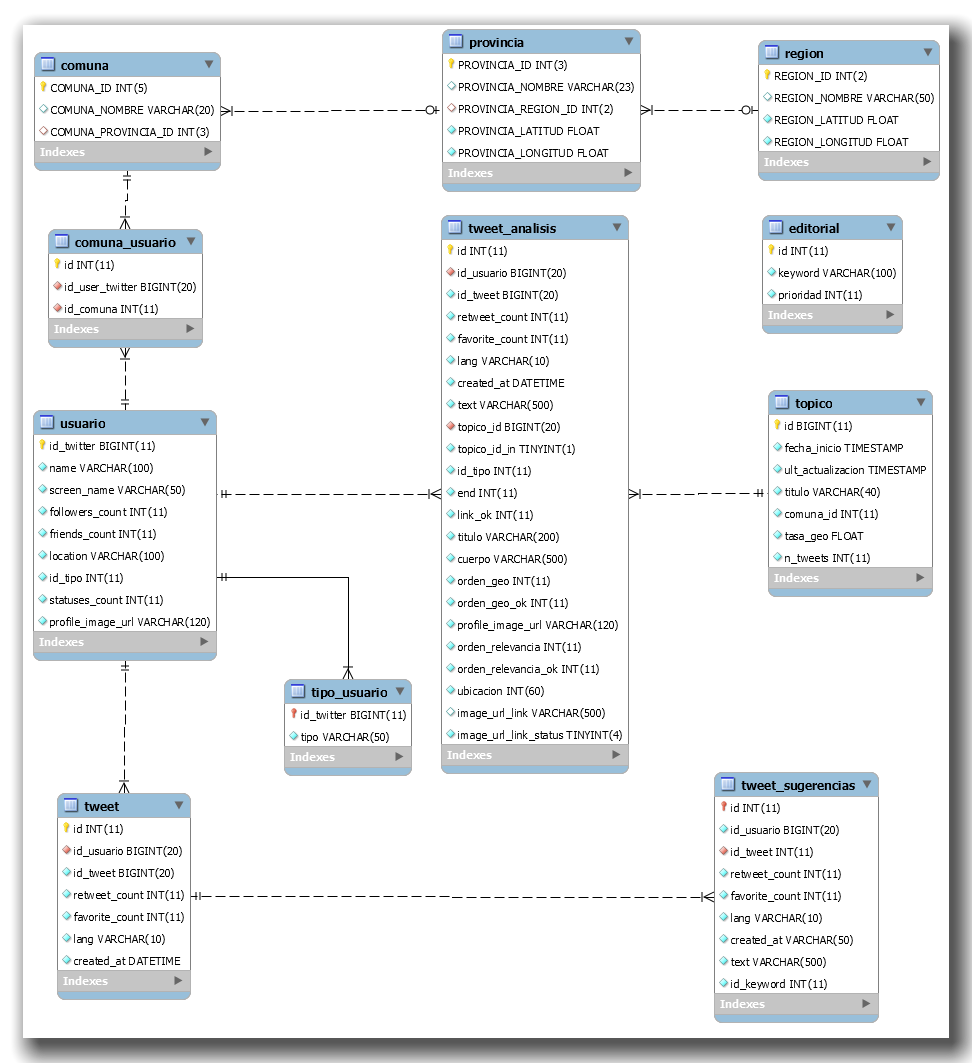
\includegraphics[width=\textwidth]{imgs/modelo_bd.png}
  \caption{Modelo de base de datos}
  \label{fig:modelo_bd}
\end{figure}


\subsection{Análisis de la línea editorial del medio objetivo}
	Para tener una directriz respecto a qué tópicos de noticias son cubiertos por el medio de prensa objetivo, se realiza un análisis de los tweets de dicho medio.
El proceso se realiza mediante el conteo de la frecuencia de las palabras contenidas en los corpus de los distintos tweets, sin considerar las palabras vacías o stopword\footnote{Stopwords o palabras vacías es el nombre que reciben las palabras sin significado como artículos, pronombres, preposiciones, etc. que son filtradas antes o después del procesamiento de datos en lenguaje natural (texto)} presentes.

\begin{algorithm}
	\caption{Obtención de las palabras más frecuentes del timeline de un conjunto de tweets}\label{ciudadesLeven}
	\begin{algorithmic}[1]
		\Function{getKeywordMedio}{tweets}
		\For{tweet in tweets}
		\For{tweet in tweets}
		\For{palabra in tweet}
		\If{stopwords.not\_in\_array(palabra)}
		\State palabras.push(palabra)
		\State frecPalabras[palabra]++
		\EndIf
		\EndFor
		\EndFor
		\EndFor
		\State return frecPalabras.ordenar()
		\EndFunction
	\end{algorithmic}
\end{algorithm}


%La cuenta de Twitter de AmorTv (\@amor\_tv) al momento de realizar la extracción con más de mil tweets de los cuales se obtuvieron los siguientes resultados:

\begin{table}[H]
	\begin{center}
		\begin{tabular}{| c | c |}
			\hline
			Posición & Palabra \\ \hline
			1 & Estudiantes \\ \hline
			2 & Valparaíso \\ \hline
			3 & Universidad \\ \hline
			4 & Toma \\ \hline
			5 & Sede \\ \hline
			6 & Represión \\ \hline
			7 & Marcha \\ \hline
			8 & Chile \\ \hline
			9 & Concepción \\ \hline
			10 & Casa Central \\ \hline
			11 & Usm  \\ \hline
			12 & Utfsm \\ \hline
			13 & Paro \\ \hline
			14 & Nacional \\ \hline
			15 & Carabineros \\ \hline
			16 & Movimiento \\ \hline
			17 & Pucv \\ \hline
			18 & Asamblea \\ \hline
			19 & Trabajadores \\ \hline
			20 & Secundarios \\ \hline
		\end{tabular}
		\caption{Tabla que muestra en orden descendente las keyword con mayor frecuencia
			en el análisis del timeline de Twitter de Amor TV}
		\label{tab:xyz}
	\end{center}
\end{table}

Se obtiene que las palabras con mayor frecuencia tienen relación con temáticas estudiantiles, manifestaciones, movimientos sociales y los lugares donde estos ocurren, que va acorde a la descripción del medio \cite{amorTV}.

%Tras el posterior análisis con los editores y miembros de amor\_tv sobre las keyword
%que con su conocimiento experto podían considerar, al momento de buscar un evento 
%noticioso agregaron las siguientes:

%	\begin{table}[h]
%	\begin{center}
%	   \begin{tabular}{| c | c |}
%		 \hline
%		   Posición & Palabra \hline
%		   1 & Trabajadores & 
%		   2 & Social & 
%		   3 & Sexismo & 
%		   4 & Santa Maria & 
%		   5 & Protesta & 
%		   6 & Movimiento & 
%		   7 & Movilización & 17 & - \\ \hline
%		   8 & Mapuche & 18 & - \\ \hline
%		   9 & Estudiantil & 19 & - \\ \hline
%		   10 & Ecológico & 20 & - \\ \hline
%		   11 & Confech  \\ \hline
%		   12 & Comunidad \\ \hline
%		   13 & Comunitario \\ \hline
%		   14 & Indígena \\ \hline
%		   15 & Autogestión \\ \hline
%		   16 Medioambiente - \\ \hline
%		\end{tabular}
%		\caption{Tabla que muestra en orden descendente las keyword con mayor frecuencia
%				en el análisis del timeline de Twitter de \@amor\_tv}
%		\label{tab:xyz}
%		 \end{center}
%	 \end{table}

%Las keyword consideradas que representan a mayor cabalidad los eventos noticiosos que
%caracterizan al medio de comunicación de prensa AmorTv, obtenidas de los análisis
%anteriores agregando variaciones de algunas palabras, son representadas gráficamente
%mediante el siguiente wordcloud:

%\begin{figure}[H]
%  \centering
%    \includegraphics[width=0.99\textwidth]{wordcloud.png}
%  \caption{WordCloud de las keyword mas representativas de los eventos noticiosos
%  característicos de AmorTv}
%  \label{fig:storyful}
%\end{figure}

\newpage

\subsection{Geolocalización de usuarios}\label{sec:geo}
\label{subsec:geo1}
	El método implementado utiliza el concepto de la distancia de Levenshtein\footnote{La distancia de Levenshtein corresponde a la cantidad de cambios necesarios en un string para transformarlo en un string objetivo.} para determinar si el texto proporcionado por el usuario como ubicación corresponde o no a una comuna existente en Chile. La información relativa a las actuales comunas, provincias y regiones de acuerdo al Decreto Exento Nº 817, del Ministerio del Interior, publicado en el Diario Oficial del 26 de Marzo de 2010 \cite{listaCodigosProvincias}. La posición GPS de cada una de las provincias se obtuvo mediante la ubicación proporcionada en \cite{dicesmapas}.

\begin{algorithm}
	\caption{Reconocimiento de ubicación del usuario mediante Levenshtein}\label{ciudadesLeven2}
	\begin{algorithmic}[1]
		\Function{getDistanciaLeven}{usuarios}
		\For{usuario in usuarios}
		\State usuario.ubicacion = limpiarPuntuacion(usuario.ubicacion)\;
		\State usuario.ubicacion = quitarNacionalidad(usuario.ubicacion)\;
		\For{comuna in comunas}
		\State dist = Levenshtein(comuna, usuario.ubicacion)\;
		\If{dist\textless MinimaDistancia}
		\State usuario.comuna = comuna\;
		\EndIf
		\EndFor
		\EndFor
		\EndFunction
	\end{algorithmic}
\end{algorithm}

%\begin{algorithm}
%	\caption{Reconocimiento de ubicación del usuario mediante SQL}\label{ciudadesSql}
%	\begin{algorithmic}[1]
%		\For{comuna in comunas}
%			\State usuariosComuna = getUsersFromBd(comuna)
%			\For{usuario in usuariosComuna}
%				\State usuario.comuna = comuna
%			\EndFor
%		\EndFor	
%	\Function{getUsersFromBd}{comuna}
%		\State sql = 'SELECT usuario WHERE usuario.ubicacion LIKE "\%" + comuna;
%		\State return execute(sql);
%	\EndFunction	
%	\end{algorithmic}
%\end{algorithm}

\subsubsection{Prueba valores distancia Levenshtein para identificar ubicación}

Para obtener cual es la distancia de Levenshtein con mejores resultados se consideró una muestra representativa de 383 usuarios elegidos de manera aleatoria y cuyo campo ubicación fuese distinto a vacío. Los resultados obtenidos fueron los siguientes:

\begin{table}[H]
	\centering
	\begin{tabular}{| c|c|c|c|}
		\hline
		D. Levenshtein & Nº match correctos & Nº match incorrectos  &  Error porcentual \\ \hline
		1   & 157 & 157 & 0,00\% \\ \hline
		2   & 172 & 164 & 2,09\% \\ \hline
		3	& 207 & 189 & 4,70\% \\ \hline
		4	& 223 & 192 & 8,09\% \\ \hline
		5	& 235 & 194 & 10,70\% \\ \hline
	\end{tabular}
	\caption {Tabla comparativa para distintas valores de distancia de Levenshtein}
\end{table}

Podemos observar que a medida que aumentamos la distancia de Levenshtein, va aumentando la cantidad de coincidencias correctas pero también la cantidad de falsas coincidencias que ocurren.

Se consideró que un error menor al 5\% es adecuado, considerando la cantidad de coincidencias correctas que aporta al conjunto. Por lo anterior se concluye que la distancia de Levenshtein a utilizar corresponde a 3. Considerando este parámetro el número de coincidencias entre el campo ubicación y los nombre estándar de las comunas es de 114.016 del total de 650.000 usuarios (correspondiente al 17,54\% de usuarios). Éste porcentaje comparativamente es mayor que el 12\% encontrado en \cite{Cheng:2010:YYT:1871437.1871535} por Cheng mediante su primera metodología explicada en  \ref{sebsec:geoestadoarte}.

Al disponer los distintos usuarios en un mapa utilizando la API de mapas de Google, se obtienen la siguiente visualización:

\begin{figure}[H]
	\centering
	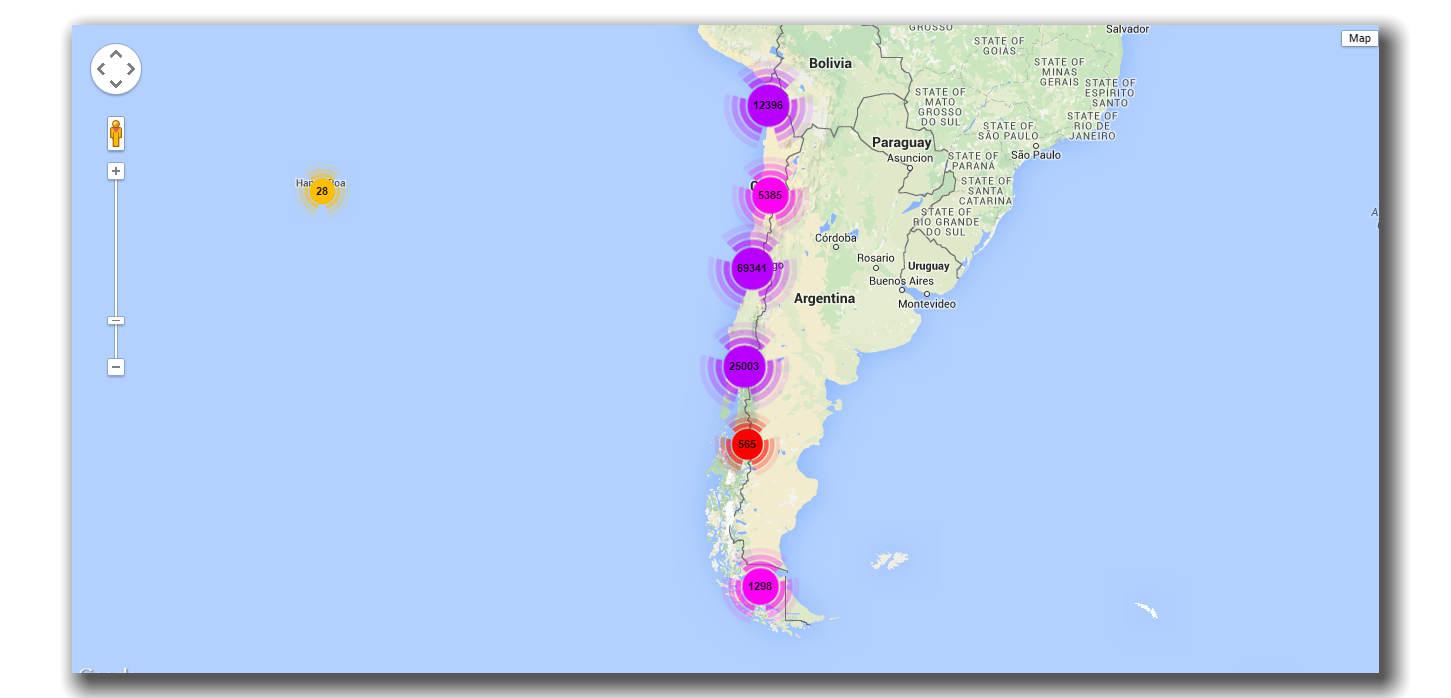
\includegraphics[width=0.9\textwidth]{imgs/mapa_usuarios.png}
	\caption{Mapa con los usuarios por ubicación geográfica}
	\label{fig:mapa_usuarios}
\end{figure}


\newpage
\subsection{Captación de usuarios}

El proceso de captación del conjunto de usuarios esta diseñado con la intención de obtener todas y todos los usuarios residentes en territorio Chileno dado que dicho catastro no existe en ninguna fuente oficial actualizada. El procedimiento se basa en las siguientes dos consideraciones: c
\begin{enumerate}
	\item Los generadores de información poseen una gran base de seguidores \cite{JavaEtAl:07}.
	\item Es habitual que los seguidores de medios de prensa al querer difundir una información le escriban un tweet a algún medio de prensa o figura de autoridad, esperando que este realice un re-tweet, para llegar también a su base de seguidores.
\end{enumerate}

El proceso de construcción de la lista de usuarios se componen de dos grandes etapas, las cuales son explicadas a continuación:

\begin{figure}[H]
	\centering
	\begin{tikzpicture}[node distance = 2cm, auto]
	
	\node [block, node distance=2.5cm, minimum width=9em, text width=8em] (i1) {\textsf{Captura de medios de prensa (MP)}};
	\node [block, below of=i1, node distance=2.5cm, minimum width=9em, text width=8em] (i2) {\textsf{Captura followers de los Medios de prensa(FMP)}};
	
	% Draw edges
	\path [line] (i1) -- (i2);
	
	\end{tikzpicture}
\caption{Diagrama conceptual con las etapas para la captación de usuarios.} \label{fig:etapas-captacion-usuarios}
\end{figure}

\subsubsection{Captura de los medios de prensa (MP)}

Para generar la lista de medios de prensa (MP) se accede a los medios de prensa registrados en las tres asociaciones más grandes de medios de comunicación de Chile:
\begin{itemize}
	\item \textit{ANP (Asociación Nacional de Prensa)} \cite{anpWebsite}: Asociación gremial constituida el 24 de agosto de 1951. Agrupa a los principales diarios y revistas del país.
	\item \textit{ANARCICH (Asociación nacional de Radios Comunitarias y Ciudadanas de Chile)} \cite{anarcichWebsite}: Es el organismo que agrupa a 300 radios comunitarias y ciudadanas de todo el país. 
	\item \textit{ARCHI (Asociación de Radiodifusores de Chile)} \cite{archiWebsite}: Fundada en 1933 es la organización gremial de medios de comunicación social más antigua de Chile.
\end{itemize}	

Ninguna de las asociaciones de medios de prensa considerados anteriormente (ANP, ANARCICH y ARCHI) cuentan con directorios públicos \cite{mediosArchi} \cite{mediosaAnp} \cite{mediosAnarcich} que provean las cuentas oficiales de Twitter de los diversos medios. Por lo cual, para recolectarlas se implementa el siguiente algoritmo ejecutado por un ser humano:

\begin{algorithm}[H]
	\caption{Construcción lista de medios}\label{mediosPrensa}
	\begin{algorithmic}[1]
		\Function{getTwitterAccount}{listaMedios}
		\For{medio in listaMedios}
		\State busqueda $\gets$ 'site:twitter.com'+medio.nombre+medio.tipo +'chile'
		\State resultGoogle $\gets$ BusquedaGoogle ( busqueda, $limit=12$)
		\For{result in resultGoogle}
		\If{result.title \&\& result.description se relacionan con medio  }
		\State medio.screenName $\gets$ result.screenName
		\EndIf 
		\EndFor
		\EndFor
		\State return listaMedios
		\EndFunction	
		%	\Function{getUsersFromBd}{comuna}
		%		\State sql = 'SELECT usuario WHERE usuario.ubicacion LIKE "\%" + comuna;
		%		\State return execute(sql);
		%	\EndFunction	
	\end{algorithmic}
\end{algorithm}

Tras aplicar este algoritmo, los resultados obtenidos fueron los siguientes:

\begin{table}[H]
	\centering
	\begin{tabular}{|c|c|c|}
		\hline
		Asociación & Nº asoc. con cuentas & Nº asoc. totales \\ \hline
		ANP & 43 & 93 \\ \hline
		ANARCICH & 23 & 99 \\ \hline
		ARCHI & 9 & 304 \\ \hline
	\end{tabular}
	\caption {Cantidad de miembros de las distintas asociaciones de prensa en Chile con cuentas en Twitter al 5 de junio del 2014.}
\end{table}


\subsubsection{Captura followers de los medios de prensa (FMP)}

Tras obtener la lista de medios de prensa, mediante la API de Twitter se recopilan los seguidores de cada uno de los medios de prensa. El algoritmo continuación realiza esta tarea requiere de realizar pero debe incluir intervalos de pausas para respetar las restricciones de número de solicitudes por hora que impone la API.

\begin{algorithm}[H]
	\caption{Captura de usuarios}\label{capturaUsuarios}
	\begin{algorithmic}[1]
		\Function{GetPop}{mediosPrensa}
		\For{medio in mediosPrensa} 
		\If{GetFriendsInformation(medio, api)}
		\State Sleep(2);
		\Else
		\State Sleep(60*15);
		\State GetFriendsInformation(medio, api)
		\EndIf
		\EndFor
		\EndFunction
		
		\Function{GetFriendsInformation}{user, api}	
		\State TwitterFriends $gets$ api.GetFollowers(screenName=user)
		\If {TwitterFriends.length > 0}
		\For {Friends in TwitterFriends}:
		\State SaveInBd(Friends)
		\EndFor
		\Else
		\State Sleep(60*15);
		\EndIf
		\EndFunction
		
	\end{algorithmic}
\end{algorithm}

Una de las dificultades presentadas en el algoritmo anterior, era que ante usuarios con más de 1,5 millones de seguidores la petición a la API se demoraba un tiempo excesivo (más de 48 horas) y retornaba error por \emph{timeout} de la conexión. Para sortear esta dificultad fue necesario modificar la API Python Twitter directamente, agregando el retorno del cursor aún cuando se agota la conexión con la API y guardando los resultados parciales de las respuestas. El cursor de una llamada en la API es similar a un índice que permite realizar solicitudes de manera segmentada a la API \footnote{ Al día 26/10/2015 no se encontraba disponible la mejora en el \emph{Github} oficial de la librería \cite{pythonTwitterGithub} }. Esta modificación fue realizada en base a las recomendaciones y comentarios disponibles en los grupos de desarrolladores de la librería \cite{pythonTwitterCode} \cite{pythonTwitterGithub}. 


	\begin{algorithm}[H]
			\caption{GetFollowers}\label{getFollowers}
			\begin{algorithmic}[1]
			    \Function{GetFollowers}{self, screen\_name=None, cursor=-1}
			    \State result $\gets$ []
			    \State parameters $\gets$ \{\}
			    \While{True}: \label{getFollowers:line:line4}
				    \State next\_cursor, previous\_cursor, data $\gets$ api.GetFollowersPaged(user\_id, screen\_name, cursor)
				    \State result += [User.NewFromJsonDict(x) for x in data['users']]
				    \If{next\_cursor == 0 or next\_cursor == previous\_cursor}\label{getFollowers:line:line7}
					    \State break
				    \Else
					    \State cursor $\gets$ next\_cursor
				    \EndIf
				    \State sec $\gets$ self.GetSleepTime('/followers/list')
				    \State time.sleep(sec)
			    \EndWhile
				    \State return result
				\EndFunction				
			\end{algorithmic}
		\end{algorithm}

		\begin{algorithm}[H]
			\begin{algorithmic}[1]
				\Function{GetFollowers}{self, screen\_name=None, cursor=-1}:
					\State result $\gets$ []
					\State parameters $\gets$ \{\}
				%\If{screen\_name is not None}:
				%\State parameters['screen\_name'] $\gets$ screen\_name
				%\EndIf
				%\State parameters['include\_user\_entities'] $\gets$ True
				\color{orange}
				\State remaining $\gets$ 15
				\State ratelimited $\gets$ False
				\While{remaining $>$ 1}
					\State remaining $\gets$ remaining-1
					\State parameters['cursor'] $\gets$ cursor
					\color{black}
					\State json $\gets$ api.\_RequestUrl(url, 'GET', data=parameters)
					\State data $\gets$ api.\_ParseAndCheckTwitter(json.content)
					\If{data}
							\State result $+=$ [User.NewFromJsonDict(x) for x in data['users']]
						\If {'next\_cursor' in data}:
							\If {data['next\_cursor'] == 0 \\ OR data['next\_cursor'] == data['previous\_cursor']}
								\State break
							\Else:
								\State cursor $\gets$ data['next\_cursor']
							\EndIf
						\Else:
							\State break
						\EndIf
						\Else
						\color{orange}
							\State ratelimited $\gets$ True
							\State break
					\EndIf
					
				\EndWhile
				\State return (cursor, result, ratelimited)
				\color{black}
				\EndFunction
				
			\end{algorithmic}
			\caption{GetFollowers con mejora}\label{getFollowerModif}
		\end{algorithm}

La modificación relacionadas a la dificultad mencionada anteriormente se pueden observar en el algoritmo \ref{getFollowerModif} donde fueron resaltadas con otro color. Principalmente incorpora un límite de llamadas a la API a 15 llamadas consecutivas de tal manera de reducir el intervalo de respuesta de la llamada, este parámetro fue determinado en base a la restricción de la API de Twitter. Esta modificación permite ir guardando nuevos datos de manera frecuente sin necesidad de esperar hasta completar todos los followers de un usuario. En  la función original las líneas ~\ref{getFollowers:line:line4} y ~\ref{getFollowers:line:line7} mantienen el ciclo de consultas por followers hasta que los cursores indican que no existen más followers por recibir (y sólo cumplida esa condición retorna datos).

El algoritmo se demora en promedio 2,6945531 segundos en descargar los datos de un usuario y almacenarlos en el sistema.

\subsection{Captura de tweets}

El proceso de captura de tweets se realiza obteniendo los 100 últimos tweets de cada uno de los usuarios y usuarias recolectadas en la fase anterior, sin discriminación ni priorización alguna, tal como muestra el siguiente algoritmo:

\begin{algorithm}[H]
	\caption{Algoritmo para la captura de tweets.}\label{getTweets}
	\begin{algorithmic}[1]
		\Function{GetTweets}{}
		\State usuarios $\gets$ getUsersFromBD();
		\For {usuario in usuarios}
		\State GetUserTimeline(id\_user=usuario.id);
		\EndFor
		\State time.sleep(5);
		\EndFunction
		
		\Function{GetUserTimeline}{id\_user}:
		\State statuses $\gets$ api.GetUserTimeline(user\_id=id\_user,count=100);
		\State SaveTweetInBD(statuses);
		
		\If {statuses.error == 34}
		\Comment{La cuenta ya no existe}
		\State return 1;
		\EndIf
		
		\If {statuses.error == 179}
		\Comment{La cuenta es privada}
		\State return 1;
		\EndIf
		
		\If {statuses.error == 88}
		\Comment{Limite de solicitudes excedidas}
		\State time.sleep(5*60);
		\State return
		\EndIf
		\EndFunction
	\end{algorithmic}
\end{algorithm}

El algoritmo planteado principalmente en su primera etapa realiza una búsqueda de los usuarios y sus respectivos estados referentes a si han sido recolectados sus últimos tweets (en cuyo caso se van a buscar los 100 tweets más recientes a partir del último recogido) o no (en cuyo caso se van a buscar los 100 tweets más recientes), posteriormente se almacenan en la base de datos los tweets recibidos. Es importante resaltar que este algoritmo gestiona las distintas pausas necesarias para respetar los límites de la API Twitter y posibles restricciones sobre si la cuenta no existe o es privada. 

El algoritmo se demora en promedio 0,9658139 segundos en descargar los tweets de un usuario y almacenarlos en el sistema.

\subsection{Procesamiento de los tweets}

El procesamiento de los tweets se define en tres procesos:
\begin{enumerate}
	\item{Definición del tópico.}
	\item{Obtención del conjunto de tweets relacionados al tópico.}
	\item{Depuración de conjunto de tweets relacionados al tópico.}
\end{enumerate}

\subsubsection{Definición del tópico}

Un tópico son las palabras claves que definen una búsqueda temática realizada por el administrador del sistema mediante la plataforma web, cada tópico posee los siguientes atributos:
\begin{itemize}
	\item \textit{Fecha de inicio} : Se refiere a la fecha de inicio de emisión de los tweets objetivos que se requiere reunir.
	\item \textit{Fecha última actualización}: Se refiere a la última fecha en la cual se realizó alguna modificación referente al tópico.
	\item \textit{Título}: Se refiere a las palabras claves que definen al tópico. 
	\item \textit{Comuna}: Comuna relacionada al tópico.
	\item \textit{Tasa de contenidos georeferenciados}: Relación entre tweets con relación geográfica y los tweets totales.
	\item \textit{Cantidad de tweets relacionados}: Total de tweets depurados del conjunto de tweets relacionados. 
\end{itemize}

\subsubsection{Obtención del conjunto de tweets relacionados al tópico}

Para obtener el conjunto de tweets relacionados al tópico se realiza una búsqueda en todos los tweets emitidos durante el periodo de interés
y que contengan las palabras claves que definen al tópico. Posteriormente se eliminan los tweets que poseen una similitud 0.85\% en sus textos 
utilizando la librería \emph{difflib}. Esta consulta se demora entre 30 y 130 segundos.

\begin{algorithm}[H]
	\caption{Obtención del conjunto de tweets relacionados al tópico}\label{getTweetsKeyword}
	\begin{algorithmic}[1]
		
		\Function{getTweetKeyword}{keywords,fecha}:
		%\Comment{Query tematica: va a buscar tweets que contengan una cierta keyword y retorna un array con las palabras que la contengan}
		\State tweets $\gets$ getTweetsFromBD(keywords, fecha);
		\State tweets $\gets$ eliminacionTweetsRepetidos(tweets);
		\State return tweets
		\EndFunction
	\end{algorithmic}
\end{algorithm}	



\subsubsection{Depuración de conjunto de tweets relacionados al tópico}

El proceso de depuración del conjunto de tweets obtenidos en el proceso anterior considera dos etapas distintas dependiendo del volumen de los tweets involucrados.

Un gran desafío en la depuración de los tweets, es discernir si un tweet en particular se relaciona o no con la temática del tópico, o por el contrario, si responde a una temática completamente distinta (y fue relacionado con el tópico únicamente por concordancia textual). Por ejemplo, si el tópico se refiere a "la paralización del registro civil", con la keyword 'paro' se busca excluir todos los tweets que se refieran a un "paro cardíaco" o de "la acción de levantarse".

Para aplicar un filtro efectivo se consideran las siguientes premisas:
\begin{itemize}
	\item El administrador del sistema posee poco tiempo (una tarea como eliminar filtros es un trabajo repetitivo y monótono, que requiere varias horas hombres para su desarrollo).
	\item Es fundamental filtrar con precisión los tweets que no corresponden a la temática.
\end{itemize}

Para conjuntos de tweets de menos de 300 tweets se considera que su depuración puede ser realizada de manera manual, debido a que no es un gran conjunto de datos y su análisis manual no demanda tiempo excesivo.

Para conjuntos de 300 tweets o más se considera que su depuración manual es muy extensa y debe ser automatizada. Para su automatización se implementa un clasificador de Bayes-Naive. El clasificador Bayes-Naive utilizado es una implementación de la librería Python Textblob \cite{textblobWebsite}.

Los tamaños de los distintos conjuntos dependiendo del tamaño del conjunto de tweets es el siguiente:

\begin{table}[h]
	\centering
	\begin{tabular}{| c | c | c |}
		\hline
		Nº tweets & Nº Entrenamiento & Nº Validación \\ \hline
		N $\leqslant$ 300	& Manual & Manual \\ \hline
		0 $\leqslant$ N $\leqslant$ 430	& N $*$ 0,2 & N*0,3	\\ \hline
		430 $\leqslant$ N & 200 & 100	\\ \hline
	\end{tabular}
	\caption {Cantidades conjuntos del clasificador utilizado}
\end{table}

Estas cantidades fueron determinadas de manera empírica en base a recomendaciones recogidas en foros y experimentos propios realizados con la librería de tal manera de obtener una precisión de clasificación siempre superior a 85\%.

\begin{algorithm}
	\caption{Clasificador Bayes-Naive para determinar si es miembro o no del tópico.}\label{CrearClasificador}
	\begin{algorithmic}[1]
		\Function{crearClasificador}{}
		\State restoTweets, tweetsValidacion, tweetsEntrenamiento $\gets$ SepararConjuntos(tweets);
		\State clasificador.entrenar(tweetsEntrenamiento)
		\State clasificador.validar(tweetsValidacion)
		
		\For {tweet in restoTweets}
			 \State clasificador.clasificar(tweet);
		\EndFor
		\EndFunction
	\end{algorithmic}
\end{algorithm}

	

La clasificación de los distintos tweets en las categorías \emph{pertenece al tópico} y \emph{no pertenece al tópico} se realiza mediante la función \emph{prob\_classify(tweet).max()} que retorna la etiqueta de la clasificación que posee mayor probabilidad según el clasificador para el tweet en específico \cite{naivebayesdoc}.

\subsubsection{Orden geográfico}

El orden geográfico dota al prototipo de un filtro que privilegia a las fuentes cercanas al lugar indicado como origen del hecho noticioso en desmedro de aquellas que se ubican a mayor distancia geográfica.

El orden geográfico se basa en la posición geográfica del autor de cada tweet analizado  en la sección ~\ref{subsec:geo1}. Inicialmente se obtienen las comunas con menor distancia a la comuna central determinada como origen del tópico y se aumenta progresivamente la distancia hasta clasificar todos los tweets de autores geoposicionados, los tweets sin ubicación son desplazados al final del ranking. 

\begin{algorithm}[H]
	\caption{Orden Geográfico}\label{OrdenGeo}
	\begin{algorithmic}[H]
		\Function{ordenGeografico}{comunaCentral}
		\State d $\gets$ 0
		\State i $\gets$ 0
		\State tweets $\gets$ getTweetsUbicados()
		\While{todosAsignados(tweets) == false}
			\State comunas $\gets$ getComunasFromDistance(d, comunaCentral)
			\For{comuna in comunas}
				\State tweets $\gets$ getTweetsFromComuna(comuna)
				\For{ tweet in tweets}
					 \State tweet.ordenGeo $\gets$ i
					 \State i $\gets$ i + 1
				\EndFor
			\EndFor
			\State d $\gets$ d + 1
		\EndWhile
		\EndFunction	
	\end{algorithmic}
\end{algorithm}


\subsubsection{Orden de relevancia}\label{subsubsec:orden-rel} 	

El objetivo de este \emph{ranking}, es generar un mecanismo que ordene los contenidos en base a su relevancia, entendida como el grado de utilidad de un tweet para informar al usuario respecto al evento en cuestión.

Para su diseño se considera la cantidad de re-tweets con que cuenta el tweet basado en el razonamiento abordado en \cite{conf/cikm/UysalC11} donde se considera que la acción de re-tweet resumen en un solo indicador, la importancia que le atribuyen sus lectores al contenido del tweet y lo replican, porque lo consideran relevante y en el estudio de la intención realizado en \cite{Yamaguchi:2010:TTU:1991336.1991364} referente a que si la intención del re-tweet es difundir (intención buscada por el prototipo, tweets que busquen informar y difundir sobre el tópico), es bastante probable que posea una gran cantidad de re-tweet, no así los tweets conversacionales .
 
 En el diseño también se considera la fecha de emisión del tweet, implementando un sistema de tres clasificaciones basado en el ranking desarrollado en \cite{Dong:2010:TEI:1772690.1772725} con la diferencia que se utilizan tres grados de clasificación y no cinco.

El mecanismo de descenso implementado considera que un tweet esta \emph{fuera de la fecha} cuando la fecha de emisión del tweet es 4 días antes que la fecha de emisión del tweet más reciente del conjunto de tweets y considera que un tweet esta totalmente \emph{fuera de fecha} cuando la fecha de emisión del tweet es 10 o más días antes que la fecha de emisión del tweet más reciente del conjunto. Para los tweets \emph{fuera de fecha} se aplica un descenso de una categoría, mientras que para los tweets \emph{totalmente fuera de fecha} se aplica un descenso de dos categorías.

\begin{algorithm}[H]
	\caption{Orden Relevancia}\label{OrdenRel}
	\begin{algorithmic}[1]
		\Function{ordenRelevancia}{}
		\State maxRT $\gets$ getMaxRT()
		\State minRT $\gets$ getMinRT()
		\State fechaMasReciente $gets$ getFechaMasReciente()
		\State firstClass, secondClass, thirdClass $gets$ dividirConjuntoPorRT(tweets)
		
		\For{ tweet in firstClass}
		\State deltaFecha $\gets$ diff(fechaMasReciente, tweet.fecha)
		
		\If{ deltaFecha $\geqslant$ 4 dias}
			\State tweet.clase $\gets$ tweet.clase - 1
			\ElsIf { deltaFecha $\geqslant$ 10 dias}
				\State tweet.clase $\gets$ tweet.clase - 2
		\EndIf
		
		\EndFor
		
		\For{ tweet in secondClass}
		\State deltaFecha $\gets$ diff(fechaMasReciente, tweet.fecha)
			\If{ deltaFecha $\geqslant$ 4 dias}
				\State tweet.clase $\gets$ tweet.clase - 1
			\EndIf
		\EndFor	
		\EndFunction
	\end{algorithmic}
\end{algorithm}

%\emph{Resultados}
	
%	Para realizar experimentos con este orden se seleccionaron X tweets de forma aleatoria de un topico determinado, estos tweets fueron presentados de forma aleatoria en un formulario de papel en donde por cada tweet se presentaba:
	
%	\begin{itemize}
%		\item Texto del tweet
%		\item Fecha del tweet
%	\end{itemize}
	
%	Las instrucciones del formulario para cada evaluador experto indicaba: \emph{Ordene los siguientes textos de tweets, colocando un numero en la linea ubicada a la derecha de cada texto, según su relevancia (grado de utilidad del tweet para informar al usuario respecto al evento en cuestión) }. Los resultados obtenidos fueron los siguientes:
	
%	\input{result-orden-rel.tex}
		

\subsubsection{Panel de enlaces}

Esta vista fue desarrollada con la intención de crear una sección de \emph{bibliografía multimedia} de un tópico. Mediante un algoritmo que recoge todos los enlaces compartidos mediante los tweets del tópico y los presenta a modo
de grilla.

Esta vista permite en mismo espacio, acceder a enlaces externos que permiten extender la información del tópico aportada por los distintos tweets, así como acceder a enlaces de distintas posturas permitiendo entre otras cosas contraponer la forma en que presentan la información, profundidad, etc.

Los enlaces son ordenados en base a su tweet de origen, del más reciente al menos reciente y luego del que posee más re-tweets al que posee menos.

\begin{algorithm}
	\caption{Obtención de enlaces externos contenidos en los tweets}\label{getURLAlgo}
	\begin{algorithmic}[H]
		\Function{GetUrlsByTweets}{tweets}
		tweets $\gets$ ordenarRelevancia(tweets);
		%\State Obtener lista de tweets del topico ordenados del más reciente al menos reciente, del que posee más re-tweets al que posee menos
		\For{ tweet in tweets}
			\If{hasURL(tweet)}
				\State urls.append(tweet.url)
			\EndIf
		\EndFor
		\For{url in urls}
			\State url.titulo, url.link, url.imagen $\gets$ getInformationURL(url)
		\EndFor 
		\EndFunction

	\end{algorithmic}
\end{algorithm}

Debido a la gran versatilidad del origen que poseen los distintos enlaces compartidos, existen dificultades en su recolección por distintos motivos como: URL incorrectas o inexistentes, textos que no es posible manipular, etc.

Para capturar los datos del enlace, se utilizó la librería lxml \ref{itm:lxml} de Python, navegando por la estructura del documento HTML se extrae el título, en enlace completo y una imagen representativa. Las condiciones mínimas que se aplica a cada uno de estos datos, es que el titulo tenga más de 10 caracteres, que la imagen posea el metatag \emph{image} de Opengraph \cite{openGraphProtocol} y que el enlace no retorne error 404 (página no encontrada).


	
	   

\subsubsection{ON/OFF Medios de prensa}
El botón \emph{ON/OFF Medios de prensa} permite ocultar o mostrar todos los tweets de la lista que hayan sido emitido por una cuenta registrada en el sistema como medio de prensa. Esta funcionalidad fue desarrollada con la intención de contar con la opción voluntaria de visualizar o no, los tweets de las cadenas de prensas, para privilegiar la lectura de tweets generados por personas o entidades sociales.
